\documentclass[12pt,a4paper]{article}
\usepackage[utf8]{inputenc}
\usepackage[margin=1in]{geometry}
\usepackage{graphicx}
\usepackage{hyperref}
\usepackage{listings}
\usepackage{xcolor}
\usepackage{titlesec}
\usepackage{fancyhdr}
\usepackage{tcolorbox}
\usepackage{enumitem}
\usepackage{tikz}
\usetikzlibrary{shapes.geometric, arrows, positioning, fit, backgrounds}

% Color definitions
\definecolor{codegreen}{rgb}{0,0.6,0}
\definecolor{codegray}{rgb}{0.5,0.5,0.5}
\definecolor{codepurple}{rgb}{0.58,0,0.82}
\definecolor{backcolour}{rgb}{0.95,0.95,0.92}
\definecolor{primaryblue}{RGB}{41,128,185}
\definecolor{secondarygreen}{RGB}{39,174,96}

% Code listing style
\lstdefinestyle{mystyle}{
    backgroundcolor=\color{backcolour},   
    commentstyle=\color{codegreen},
    keywordstyle=\color{magenta},
    numberstyle=\tiny\color{codegray},
    stringstyle=\color{codepurple},
    basicstyle=\ttfamily\footnotesize,
    breakatwhitespace=false,         
    breaklines=true,                 
    captionpos=b,                    
    keepspaces=true,                 
    numbers=left,                    
    numbersep=5pt,                  
    showspaces=false,                
    showstringspaces=false,
    showtabs=false,                  
    tabsize=2
}
\lstset{style=mystyle}

% Header and footer
\pagestyle{fancy}
\fancyhf{}
\fancyhead[L]{\leftmark}
\fancyhead[R]{\thepage}
\fancyfoot[C]{Bus Tracker System - Design Document}

% Title formatting
\titleformat{\section}
  {\normalfont\Large\bfseries\color{primaryblue}}{\thesection}{1em}{}
\titleformat{\subsection}
  {\normalfont\large\bfseries\color{secondarygreen}}{\thesubsection}{1em}{}

\begin{document}

% Title Page
\begin{titlepage}
    \centering
    \vspace*{2cm}
    
    {\Huge\bfseries Bus Tracker System\\[0.5cm]}
    {\Large System Design Document\\[2cm]}
    
    \begin{tcolorbox}[colback=primaryblue!10,colframe=primaryblue,width=12cm]
        \centering
        \textbf{A Comprehensive School Bus Tracking and\\Student Attendance Management System}
    \end{tcolorbox}
    
    \vspace{2cm}
    
    {\large
    \textbf{Version:} 1.0\\[0.3cm]
    \textbf{Date:} \today\\[0.3cm]
    \textbf{Technology Stack:}\\
    FastAPI | React | MongoDB | Raspberry Pi\\[1cm]
    }
    
    \vfill
    
    {\large
    \textbf{Document Purpose:}\\[0.3cm]
    This document provides a comprehensive technical design\\
    of the Bus Tracker System architecture, components,\\
    data models, and integration patterns.
    }
    
\end{titlepage}

\tableofcontents
\newpage

% Executive Summary
\section{Executive Summary}

The Bus Tracker System is a modern, full-stack web application designed to streamline school transportation management through real-time GPS tracking, automated RFID-based student attendance, and role-based dashboards for parents, teachers, and administrators.

\subsection{Key Features}
\begin{itemize}[leftmargin=*]
    \item \textbf{Real-time Bus Tracking:} Live GPS monitoring with interactive maps
    \item \textbf{Automated Attendance:} RFID scanning with photo capture and face verification
    \item \textbf{Role-based Dashboards:} Customized interfaces for Parents, Teachers, and Admins
    \item \textbf{Instant Notifications:} Real-time alerts for identity mismatches and updates
    \item \textbf{IoT Integration:} Raspberry Pi devices with RFID readers and cameras
    \item \textbf{Backup System:} Production-ready backups with SHA256 integrity verification
\end{itemize}

\subsection{System Goals}
\begin{itemize}[leftmargin=*]
    \item Enhance student safety through real-time tracking and verification
    \item Automate attendance recording and reduce manual errors
    \item Provide instant visibility to parents on their children's status
    \item Enable efficient school transportation management
    \item Support offline operation with graceful degradation
\end{itemize}

\newpage

% System Architecture
\section{System Architecture}

\subsection{High-Level Architecture}

The Bus Tracker System follows a three-tier architecture pattern with IoT integration:

\begin{enumerate}
    \item \textbf{Presentation Layer:} React-based responsive web application
    \item \textbf{Application Layer:} FastAPI REST API server
    \item \textbf{Data Layer:} MongoDB database with async operations
    \item \textbf{IoT Layer:} Raspberry Pi devices on buses
\end{enumerate}

\subsection{Architecture Diagram}

\begin{center}
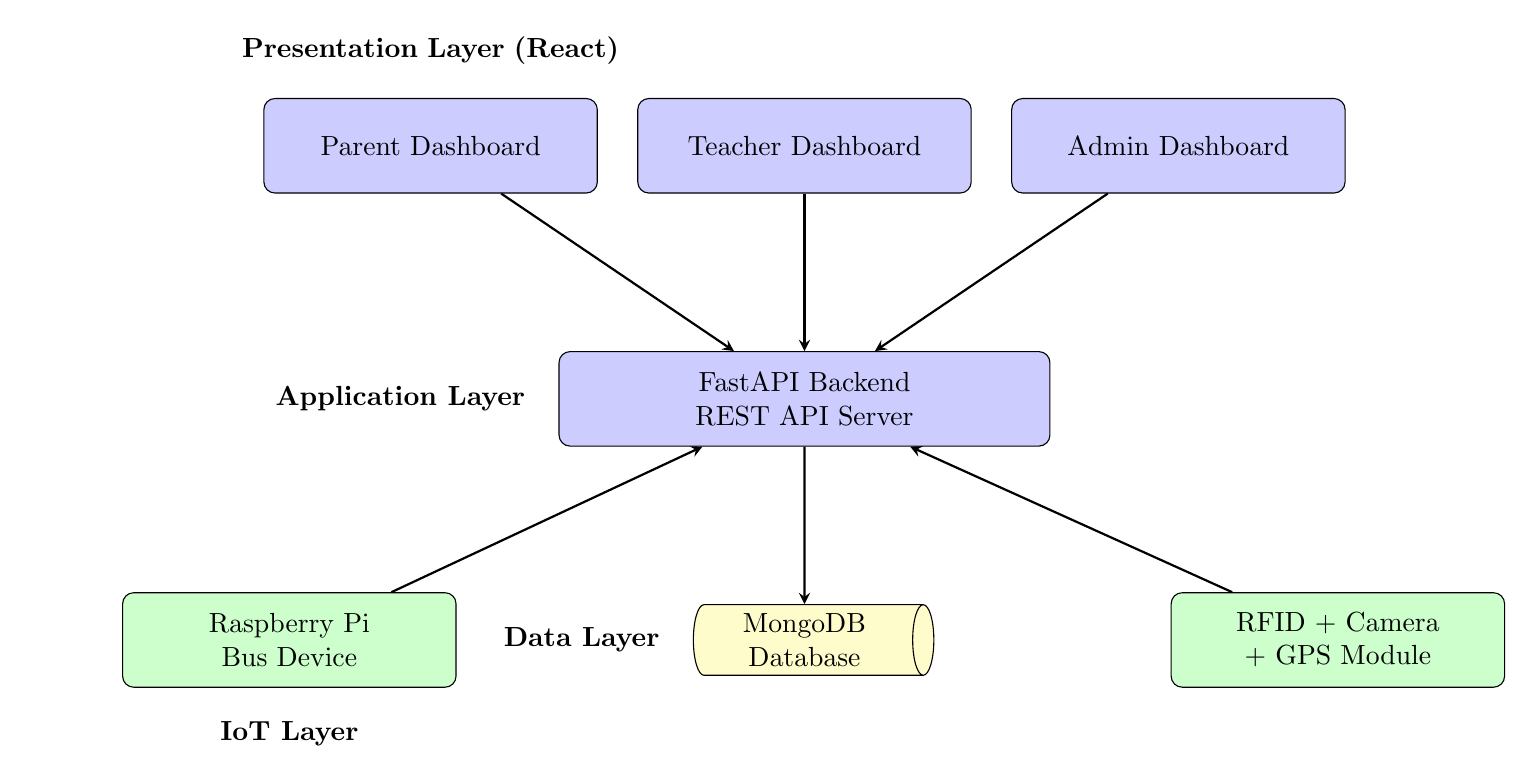
\begin{tikzpicture}[
    node distance=2cm,
    box/.style={rectangle, draw, fill=blue!20, text width=4cm, text centered, rounded corners, minimum height=1.2cm},
    iot/.style={rectangle, draw, fill=green!20, text width=4cm, text centered, rounded corners, minimum height=1.2cm},
    db/.style={cylinder, draw, fill=yellow!20, text width=2.5cm, text centered, minimum height=1.2cm, aspect=0.3},
    arrow/.style={->, >=stealth, thick}
]

% Presentation Layer
\node[box] (parent) {Parent Dashboard};
\node[box, right=0.5cm of parent] (teacher) {Teacher Dashboard};
\node[box, right=0.5cm of teacher] (admin) {Admin Dashboard};

% Application Layer
\node[box, below=2cm of teacher, text width=6cm] (api) {FastAPI Backend\\REST API Server};

% Data Layer
\node[db, below=2cm of api] (mongo) {MongoDB\\Database};

% IoT Layer
\node[iot, left=3cm of mongo] (pi1) {Raspberry Pi\\Bus Device};
\node[iot, right=3cm of mongo] (pi2) {RFID + Camera\\+ GPS Module};

% Arrows
\draw[arrow] (parent) -- (api);
\draw[arrow] (teacher) -- (api);
\draw[arrow] (admin) -- (api);
\draw[arrow] (api) -- (mongo);
\draw[arrow] (pi1) -- (api);
\draw[arrow] (pi2) -- (api);

% Labels
\node[above=0.3cm of parent, text width=10cm, text centered] {\textbf{Presentation Layer (React)}};
\node[left=0.3cm of api] {\textbf{Application Layer}};
\node[left=0.3cm of mongo] {\textbf{Data Layer}};
\node[below=0.3cm of pi1] {\textbf{IoT Layer}};

\end{tikzpicture}
\end{center}

\subsection{Technology Stack}

\begin{tcolorbox}[colback=blue!5,colframe=blue!40!black,title=Frontend Technologies]
\begin{itemize}[nosep]
    \item \textbf{Framework:} React 18.x
    \item \textbf{UI Library:} Radix UI, Tailwind CSS
    \item \textbf{Maps:} Leaflet with OpenStreetMap
    \item \textbf{State Management:} React Context API
    \item \textbf{Build Tool:} Create React App with Craco
\end{itemize}
\end{tcolorbox}

\begin{tcolorbox}[colback=green!5,colframe=green!40!black,title=Backend Technologies]
\begin{itemize}[nosep]
    \item \textbf{Framework:} FastAPI (Python 3.9+)
    \item \textbf{Database Driver:} Motor (Async MongoDB)
    \item \textbf{Authentication:} bcrypt, session-based auth
    \item \textbf{AI/ML:} DeepFace (face verification), OpenCV
    \item \textbf{Email:} aiosmtplib (async SMTP)
\end{itemize}
\end{tcolorbox}

\begin{tcolorbox}[colback=yellow!5,colframe=yellow!40!black,title=Database \& Infrastructure]
\begin{itemize}[nosep]
    \item \textbf{Database:} MongoDB 6.0+
    \item \textbf{Process Manager:} Supervisor
    \item \textbf{Web Server:} Uvicorn (ASGI)
    \item \textbf{Deployment:} Kubernetes with Ingress
\end{itemize}
\end{tcolorbox}

\begin{tcolorbox}[colback=red!5,colframe=red!40!black,title=IoT Technologies]
\begin{itemize}[nosep]
    \item \textbf{Hardware:} Raspberry Pi 3/4
    \item \textbf{RFID Reader:} MFRC522 module
    \item \textbf{Camera:} Pi Camera Module v2
    \item \textbf{GPS:} NEO-6M GPS module
    \item \textbf{Connectivity:} SIM800 GSM/GPRS module
\end{itemize}
\end{tcolorbox}

\newpage

% Data Model
\section{Data Model}

\subsection{Database Schema Overview}

The system uses MongoDB with the following collections:

\subsubsection{Users Collection}
Stores all system users (admins, teachers, parents).

\begin{lstlisting}[language=Python, caption=User Model]
{
    "user_id": "uuid",
    "email": "user@school.com",
    "password_hash": "bcrypt_hash",
    "role": "admin|teacher|parent",
    "name": "John Doe",
    "phone": "+1-555-0001",
    "photo_path": "backend/photos/parents/uuid.jpg",
    "address": "123 Main St",
    "student_ids": ["uuid1", "uuid2"],  # for parents
    "assigned_class": "5",              # for teachers
    "assigned_section": "A",            # for teachers
    "is_elevated_admin": true,          # for admins
    "created_at": "2025-01-01T00:00:00Z"
}
\end{lstlisting}

\subsubsection{Students Collection}
Stores student information with attendance tracking.

\begin{lstlisting}[language=Python, caption=Student Model]
{
    "student_id": "uuid",
    "name": "Emma Johnson",
    "roll_number": "G5A-001",
    "class_name": "5",
    "section": "A",
    "parent_id": "uuid",
    "teacher_id": "uuid",
    "bus_id": "BUS-001",
    "stop_id": "uuid",
    "rfid_tag": "E200001F9A8D0F23",
    "photo_path": "backend/photos/students/uuid/profile.jpg",
    "attendance_path": "backend/photos/students/uuid/attendance/",
    "embedding": "base64_face_embedding",
    "phone": "+1-555-1001",
    "address": "456 Oak Ave",
    "created_at": "2025-01-01T00:00:00Z"
}
\end{lstlisting}

\subsubsection{Attendance Collection}
Records all attendance events with photos.

\begin{lstlisting}[language=Python, caption=Attendance Model]
{
    "attendance_id": "uuid",
    "student_id": "uuid",
    "bus_id": "BUS-001",
    "date": "2025-01-15",
    "time_period": "AM|PM",
    "attendance_status": "yellow|green",
    "scan_time": "2025-01-15T07:30:00Z",
    "photo_url": "attendance/2025-01-15_AM.jpg",
    "verified": true,
    "confidence_score": 0.95,
    "location": {
        "latitude": 28.6139,
        "longitude": 77.2090
    }
}
\end{lstlisting}

\subsubsection{Buses Collection}
Stores bus information and current location.

\begin{lstlisting}[language=Python, caption=Bus Model]
{
    "bus_id": "BUS-001",
    "bus_number": "DL-01-AB-1234",
    "driver_name": "Michael Brown",
    "driver_phone": "+1-555-3001",
    "capacity": 40,
    "route_id": "uuid",
    "current_location": {
        "latitude": 28.6139,
        "longitude": 77.2090,
        "timestamp": "2025-01-15T08:00:00Z"
    }
}
\end{lstlisting}

\subsubsection{Routes Collection}
Defines bus routes with stops.

\begin{lstlisting}[language=Python, caption=Route Model]
{
    "route_id": "uuid",
    "route_name": "Route A - North District",
    "stop_ids": ["uuid1", "uuid2", "uuid3"],
    "map_path": [[lat1, lon1], [lat2, lon2], ...]
}
\end{lstlisting}

\subsubsection{Stops Collection}
Bus stop locations.

\begin{lstlisting}[language=Python, caption=Stop Model]
{
    "stop_id": "uuid",
    "stop_name": "Main Gate North",
    "latitude": 28.6139,
    "longitude": 77.2090,
    "order_index": 0
}
\end{lstlisting}

\subsubsection{Notifications Collection}
User notifications and alerts.

\begin{lstlisting}[language=Python, caption=Notification Model]
{
    "notification_id": "uuid",
    "user_id": "uuid",
    "type": "identity_mismatch|welcome|update",
    "title": "Identity Verification Alert",
    "message": "Face verification failed for Emma",
    "read": false,
    "created_at": "2025-01-15T07:30:00Z"
}
\end{lstlisting}

\subsubsection{Holidays Collection}
School holiday calendar.

\begin{lstlisting}[language=Python, caption=Holiday Model]
{
    "holiday_id": "uuid",
    "name": "Christmas Day",
    "date": "2025-12-25",
    "description": "National holiday"
}
\end{lstlisting}

\subsubsection{Device Keys Collection}
API keys for IoT devices.

\begin{lstlisting}[language=Python, caption=DeviceKey Model]
{
    "device_id": "uuid",
    "bus_id": "BUS-001",
    "device_name": "Pi Scanner - Bus 001",
    "key_hash": "bcrypt_hash",
    "created_at": "2025-01-01T00:00:00Z"
}
\end{lstlisting}

\subsection{Data Relationships}

\begin{itemize}
    \item \textbf{Users (Parents)} $\rightarrow$ \textbf{Students:} One-to-Many (via student\_ids)
    \item \textbf{Users (Teachers)} $\rightarrow$ \textbf{Students:} One-to-Many (via assigned\_class/section)
    \item \textbf{Students} $\rightarrow$ \textbf{Attendance:} One-to-Many
    \item \textbf{Buses} $\rightarrow$ \textbf{Routes:} Many-to-One
    \item \textbf{Routes} $\rightarrow$ \textbf{Stops:} One-to-Many
    \item \textbf{Students} $\rightarrow$ \textbf{Stops:} Many-to-One
    \item \textbf{Device Keys} $\rightarrow$ \textbf{Buses:} One-to-One
\end{itemize}

\subsection{Database Constraints}

\begin{itemize}
    \item \textbf{Unique Indexes:}
    \begin{itemize}
        \item users.email
        \item students.(class\_name, section, roll\_number) - Composite
        \item buses.bus\_number
        \item device\_keys.bus\_id
    \end{itemize}
    
    \item \textbf{Dependency Safeguards:}
    \begin{itemize}
        \item Students cannot be deleted if attendance records exist
        \item Parents cannot be deleted if students are linked
        \item Teachers cannot be deleted if students are assigned
        \item Buses cannot be deleted if students are assigned
        \item Routes cannot be deleted if buses are using them
        \item Stops cannot be deleted if students or routes reference them
    \end{itemize}
\end{itemize}

\newpage

% API Architecture
\section{API Architecture}

\subsection{REST API Design}

The backend exposes a RESTful API with the following characteristics:

\begin{tcolorbox}[colback=blue!5,colframe=blue!40!black,title=API Principles]
\begin{itemize}[nosep]
    \item \textbf{Base URL:} /api (Kubernetes ingress routing)
    \item \textbf{Authentication:} Session-based with httpOnly cookies
    \item \textbf{Authorization:} Role-based access control (RBAC)
    \item \textbf{Response Format:} JSON
    \item \textbf{Error Handling:} HTTP status codes with descriptive messages
    \item \textbf{Async Operations:} Non-blocking I/O with Motor driver
\end{itemize}
\end{tcolorbox}

\subsection{API Endpoint Categories}

\subsubsection{Authentication Endpoints}
\begin{lstlisting}
POST   /api/auth/login          # User login
POST   /api/auth/logout         # User logout
GET    /api/auth/me             # Get current user info
POST   /api/auth/verify-code    # Email verification (optional)
\end{lstlisting}

\subsubsection{Student Management}
\begin{lstlisting}
GET    /api/students                    # List students (role-filtered)
GET    /api/students/{id}               # Get student details
POST   /api/students                    # Create student (admin)
PUT    /api/students/{id}               # Update student (admin)
DELETE /api/students/{id}               # Delete student (admin)
GET    /api/students/class-sections     # Get existing class-sections
PUT    /api/students/{id}/register-rfid # Register RFID tag
\end{lstlisting}

\subsubsection{User Management}
\begin{lstlisting}
GET    /api/users           # List users (admin)
POST   /api/users           # Create user (admin)
PUT    /api/users/{id}      # Update user (admin)
DELETE /api/users/{id}      # Delete user (admin)
GET    /api/parents/all     # List all parents
GET    /api/parents/unlinked # List parents without children
\end{lstlisting}

\subsubsection{Attendance \& Tracking}
\begin{lstlisting}
POST   /api/scan_event              # Record attendance scan (device)
POST   /api/update_location         # Update bus GPS (device)
GET    /api/get_attendance          # Get attendance grid
GET    /api/get_bus_location        # Get current bus location
\end{lstlisting}

\subsubsection{Bus \& Route Management}
\begin{lstlisting}
GET    /api/buses               # List buses
GET    /api/buses/{id}          # Get bus details
POST   /api/buses               # Create bus (admin)
PUT    /api/buses/{id}          # Update bus (admin)
DELETE /api/buses/{id}          # Delete bus (admin)
GET    /api/buses/{id}/stops    # Get stops for bus route

GET    /api/routes              # List routes
GET    /api/routes/{id}         # Get route details
POST   /api/routes              # Create route (admin)
PUT    /api/routes/{id}         # Update route (admin)
DELETE /api/routes/{id}         # Delete route (admin)

GET    /api/stops               # List stops
POST   /api/stops               # Create stop (admin)
PUT    /api/stops/{id}          # Update stop (admin)
DELETE /api/stops/{id}          # Delete stop (admin)
\end{lstlisting}

\subsubsection{Notifications}
\begin{lstlisting}
GET    /api/get_notifications                 # List user notifications
PUT    /api/mark_notification_read/{id}       # Mark as read
DELETE /api/notifications/{id}                # Delete notification
\end{lstlisting}

\subsubsection{Holidays}
\begin{lstlisting}
GET    /api/admin/holidays          # List holidays
POST   /api/admin/holidays          # Create holiday (admin)
PUT    /api/admin/holidays/{id}     # Update holiday (admin)
DELETE /api/admin/holidays/{id}     # Delete holiday (admin)
\end{lstlisting}

\subsubsection{Device API (IoT)}
\begin{lstlisting}
POST   /api/device/register                     # Register device (admin)
GET    /api/device/list                         # List devices (admin)
GET    /api/students/{id}/embedding             # Get face embedding (device)
GET    /api/students/embedding-by-rfid          # Get embedding by RFID (device)
\end{lstlisting}

\subsubsection{Backup System}
\begin{lstlisting}
GET    /api/admin/backups/status       # Current backup status
GET    /api/admin/backups/list         # List all backups
GET    /api/admin/backups/health       # Backup system health
POST   /api/admin/backups/trigger      # Manual backup trigger
POST   /api/admin/backups/verify/{id}  # Verify backup integrity
POST   /api/admin/backups/restore/{id} # Restore from backup
\end{lstlisting}

\subsubsection{Photo Management}
\begin{lstlisting}
PUT    /api/users/me/photo             # Upload user photo
PUT    /api/students/{id}/photo        # Upload student photo
GET    /photos/*                       # Static file serving
\end{lstlisting}

\subsection{Authentication Flow}

\begin{enumerate}
    \item User submits credentials via POST /api/auth/login
    \item Backend validates credentials with bcrypt
    \item If valid, creates session token (UUID)
    \item Session stored in memory with user data
    \item Returns session\_token as httpOnly cookie
    \item Subsequent requests include cookie automatically
    \item Backend validates session on protected endpoints
    \item Logout clears session from memory and cookie
\end{enumerate}

\subsection{Device Authentication}

IoT devices use API key authentication:

\begin{enumerate}
    \item Admin registers device via POST /api/device/register
    \item System generates 64-character API key
    \item Key is hashed with bcrypt before storage
    \item Device includes X-API-Key header in requests
    \item Backend validates key using verify\_device\_key() dependency
    \item Device can only access device-specific endpoints
\end{enumerate}

\newpage

% Frontend Architecture
\section{Frontend Architecture}

\subsection{Component Structure}

The React frontend is organized into the following structure:

\begin{lstlisting}[language=bash, caption=Frontend Directory Structure]
frontend/
|-- src/
    |-- components/
        |-- AdminDashboardNew.jsx       # Admin dashboard
        |-- TeacherDashboardNew.jsx     # Teacher dashboard
        |-- ParentDashboard.jsx         # Parent dashboard
        |-- LoginPage.jsx               # Login page
        |-- AddStudentModal.jsx         # Student creation
        |-- EditStudentModalEnhanced.jsx # Student editing
        |-- StudentDetailModal.jsx      # Student details
        |-- AddHolidayModal.jsx         # Holiday creation
        |-- EditHolidayModal.jsx        # Holiday editing
        |-- PhotoViewerModal.jsx        # Photo viewer
        |-- UserProfileHeader.jsx       # User profile header
        |-- StudentCard.jsx             # Student card component
        |-- DeleteConfirmationDialog.jsx # Delete confirmation
        |-- HolidaysManagementModal.jsx  # Holidays management
    |-- App.js                          # Main app component
    |-- index.js                        # Entry point
    |-- index.css                       # Global styles
|-- public/
    |-- index.html
\end{lstlisting}

\subsection{State Management}

The application uses React Context API for global state:

\begin{itemize}
    \item \textbf{UserContext:} Current user session and profile
    \item \textbf{Component State:} Local state with useState hook
    \item \textbf{API Calls:} Direct fetch calls with async/await
\end{itemize}

\subsection{Dashboard Features}

\subsubsection{Parent Dashboard}
\begin{itemize}
    \item View children's information and photos
    \item Live bus tracking on interactive map
    \item Monthly attendance calendar with click-to-view photos
    \item Real-time notifications
    \item Student detail cards with bus and stop information
\end{itemize}

\subsubsection{Teacher Dashboard}
\begin{itemize}
    \item View assigned students list
    \item Today's AM/PM attendance status
    \item Search and filter students
    \item View student details and attendance history
    \item Access to route and bus information
\end{itemize}

\subsubsection{Admin Dashboard}
\begin{itemize}
    \item Complete CRUD operations for:
    \begin{itemize}
        \item Students with class-section management
        \item Users (admins, teachers, parents)
        \item Buses and routes
        \item Holidays
    \end{itemize}
    \item System statistics and overview
    \item Backup management and monitoring
    \item Device registration and management
    \item Elevated admin permissions
\end{itemize}

\subsection{UI/UX Design Principles}

\begin{tcolorbox}[colback=green!5,colframe=green!40!black,title=Design System]
\begin{itemize}[nosep]
    \item \textbf{Color Scheme:} Role-specific colors (blue for parents, teal for teachers, indigo for admins)
    \item \textbf{Typography:} System fonts with Tailwind CSS utilities
    \item \textbf{Icons:} Lucide React icon library
    \item \textbf{Responsive:} Mobile-first design with breakpoints
    \item \textbf{Animations:} Smooth transitions with Tailwind CSS
    \item \textbf{Accessibility:} ARIA labels and keyboard navigation
\end{itemize}
\end{tcolorbox}

\subsection{Map Integration}

The system uses Leaflet with OpenStreetMap for real-time bus tracking:

\begin{itemize}
    \item Bus marker with custom icon
    \item Route path polyline visualization
    \item Stop markers with popup information
    \item Auto-zoom to fit route bounds
    \item Toggle route display on/off
    \item GPS fallback indicator (red marker with question mark)
\end{itemize}

\newpage

% IoT Integration
\section{IoT Integration}

\subsection{Raspberry Pi Architecture}

Each bus is equipped with a Raspberry Pi device running custom Python software:

\begin{tcolorbox}[colback=red!5,colframe=red!40!black,title=Pi Hardware Components]
\begin{itemize}[nosep]
    \item \textbf{Main Controller:} Raspberry Pi 3 Model B+ or 4
    \item \textbf{RFID Reader:} MFRC522 (SPI interface)
    \item \textbf{Camera:} Pi Camera Module v2 (5MP)
    \item \textbf{GPS Module:} NEO-6M (UART)
    \item \textbf{Connectivity:} SIM800 GSM/GPRS module
    \item \textbf{Power:} 5V/3A adapter or vehicle power
\end{itemize}
\end{tcolorbox}

\subsection{Pi Software Architecture}

The Raspberry Pi runs three main scripts:

\begin{enumerate}
    \item \textbf{pi\_server.py:} Main boarding scanner controller
    \item \textbf{pi\_hardware.py:} Hardware backend (GPIO, RFID, Camera, GPS)
    \item \textbf{pi\_simulated.py:} Simulation backend (for testing)
\end{enumerate}

\subsection{Attendance Workflow}

\begin{enumerate}
    \item Student taps RFID card on reader
    \item Pi reads RFID tag and looks up student in local cache
    \item Camera captures student photo
    \item Pi performs face verification using DeepFace
    \item Confidence score calculated (threshold: 0.40)
    \item GPS coordinates captured
    \item Data uploaded to backend via API:
    \begin{itemize}
        \item Student ID
        \item Photo (base64 encoded)
        \item Verification status
        \item GPS coordinates
        \item Scan type (yellow or green)
    \end{itemize}
    \item Backend creates attendance record
    \item If face verification fails, notification sent to parent
\end{enumerate}

\subsection{Face Verification}

The system uses DeepFace library with Facenet model:

\begin{itemize}
    \item \textbf{Embedding Generation:} 128-dimension face embeddings
    \item \textbf{Similarity Metric:} Cosine similarity
    \item \textbf{Threshold:} 0.40 (adjustable)
    \item \textbf{Caching:} Embeddings stored locally in JSON file
    \item \textbf{Fallback:} API fetch if local embedding missing
    \item \textbf{Retry Logic:} 2 failures $\rightarrow$ fresh API fetch $\rightarrow$ 3 retries
\end{itemize}

\subsection{Offline Operation}

The Pi system supports offline operation:

\begin{itemize}
    \item Local embedding cache for face verification
    \item RFID-to-student mapping stored locally
    \item Queue system for failed uploads (future enhancement)
    \item Graceful degradation when API unavailable
\end{itemize}

\subsection{GPS Handling}

The system handles GPS failures gracefully:

\begin{itemize}
    \item \textbf{Valid GPS:} Full coordinates recorded
    \item \textbf{No GPS Fix:} Null coordinates sent, system continues
    \item \textbf{Frontend:} Displays red question mark indicator
    \item \textbf{Backend:} Accepts null latitude/longitude
\end{itemize}

\subsection{Device Security}

\begin{itemize}
    \item API key authentication for all device requests
    \item Keys stored securely in device configuration file
    \item Each device mapped to specific bus (1:1 relationship)
    \item Device can only update location for assigned bus
    \item Keys cannot be retrieved after generation
\end{itemize}

\newpage

% Security Architecture
\section{Security Architecture}

\subsection{Authentication \& Authorization}

\begin{tcolorbox}[colback=yellow!5,colframe=yellow!40!black,title=Security Layers]
\begin{itemize}[nosep]
    \item \textbf{Password Hashing:} bcrypt with automatic salt
    \item \textbf{Session Management:} In-memory sessions with UUID tokens
    \item \textbf{Cookie Security:} httpOnly, sameSite=lax, 24h expiry
    \item \textbf{Role-based Access:} Three roles with distinct permissions
    \item \textbf{Device Authentication:} API key (64-char hex) with bcrypt hashing
    \item \textbf{Input Validation:} Pydantic models for all requests
\end{itemize}
\end{tcolorbox}

\subsection{Role-based Permissions}

\begin{center}
\begin{tabular}{|l|c|c|c|}
\hline
\textbf{Feature} & \textbf{Parent} & \textbf{Teacher} & \textbf{Admin} \\
\hline
View own children & \checkmark & - & \checkmark \\
View assigned students & - & \checkmark & \checkmark \\
View all students & - & - & \checkmark \\
Create/edit students & - & - & \checkmark \\
Delete students & - & - & \checkmark \\
User management & - & - & \checkmark \\
Bus/route management & - & - & \checkmark \\
Holiday management & - & - & \checkmark \\
Device registration & - & - & \checkmark \\
Backup management & - & - & \checkmark \\
View notifications & \checkmark & \checkmark & \checkmark \\
Track bus location & \checkmark & \checkmark & \checkmark \\
\hline
\end{tabular}
\end{center}

\subsection{Data Protection}

\begin{itemize}
    \item \textbf{Encryption in Transit:} HTTPS required in production
    \item \textbf{Password Storage:} Never store plaintext passwords
    \item \textbf{API Response:} Password hashes excluded from responses
    \item \textbf{File Upload:} Type and size validation
    \item \textbf{Photo Access:} Static file serving with path validation
    \item \textbf{SQL Injection:} Protected by MongoDB (NoSQL)
    \item \textbf{XSS Protection:} React auto-escaping, CSP headers
\end{itemize}

\subsection{Backup Security}

\begin{itemize}
    \item \textbf{Integrity Verification:} SHA256 checksums for all backups
    \item \textbf{Backup Encryption:} File-level encryption (future enhancement)
    \item \textbf{Access Control:} Admin-only backup operations
    \item \textbf{Audit Trail:} All backup operations logged
    \item \textbf{Restore Validation:} Checksum verification before restore
\end{itemize}

\newpage

% Backup System
\section{Backup System}

\subsection{Backup Strategy}

The system implements a production-ready backup solution:

\begin{tcolorbox}[colback=blue!5,colframe=blue!40!black,title=Backup Features]
\begin{itemize}[nosep]
    \item \textbf{Auto-rotation:} Keeps last 10 backups, auto-deletes old ones
    \item \textbf{Integrity Checks:} SHA256 checksums for verification
    \item \textbf{Metadata Tracking:} Size, date, collection counts, status
    \item \textbf{Health Monitoring:} Last backup time, disk usage alerts
    \item \textbf{Manual Trigger:} Admin can trigger backup anytime
    \item \textbf{Restore Capability:} Full database restore with validation
    \item \textbf{Frontend Integration:} Status display in admin dashboard
\end{itemize}
\end{tcolorbox}

\subsection{Backup Process}

\begin{enumerate}
    \item Backup triggered (manual or scheduled)
    \item Generate unique backup ID (timestamp-based)
    \item Export all MongoDB collections to JSON
    \item Calculate SHA256 checksum of backup file
    \item Store metadata (size, counts, checksum)
    \item Rotate old backups (keep last 10)
    \item Update backup status in database
\end{enumerate}

\subsection{Restore Process}

\begin{enumerate}
    \item Admin selects backup to restore
    \item System verifies backup integrity (checksum)
    \item If valid, clears existing database collections
    \item Imports data from backup file
    \item Validates restore success
    \item Returns collection counts
\end{enumerate}

\subsection{Backup Monitoring}

Admins can monitor backup health via dashboard:

\begin{itemize}
    \item Last backup date and time
    \item Total number of backups
    \item Total backup storage size
    \item Backup history with individual sizes
    \item Health status indicators
    \item Disk usage warnings
\end{itemize}

\newpage

% Photo Management
\section{Photo Management}

\subsection{Photo Organization}

Photos are organized by user role and type:

\begin{lstlisting}[language=bash, caption=Photo Directory Structure]
backend/photos/
|-- students/
    |-- {student_id}/
        |-- profile.jpg              # Profile photo
        |-- attendance/
            |-- 2025-01-15_AM.jpg    # AM scan photo
            |-- 2025-01-15_PM.jpg    # PM scan photo
|-- parents/
    |-- {user_id}.jpg                # Parent photo
|-- teachers/
    |-- {user_id}.jpg                # Teacher photo
|-- admins/
    |-- {user_id}.jpg                # Admin photo
\end{lstlisting}

\subsection{Photo Upload}

\begin{itemize}
    \item \textbf{Allowed Formats:} JPEG, PNG
    \item \textbf{Size Limit:} 10 MB per file
    \item \textbf{Validation:} Content-type checking
    \item \textbf{Storage:} Local filesystem
    \item \textbf{Database:} photo\_path field stores relative path
    \item \textbf{URL Conversion:} Backend converts path to accessible URL
\end{itemize}

\subsection{Photo Serving}

\begin{itemize}
    \item \textbf{Static Files:} Mounted at /photos endpoint
    \item \textbf{Direct Access:} /photos/students/{id}/profile.jpg
    \item \textbf{Content-Type:} Automatic MIME type detection
    \item \textbf{Caching:} Browser caching enabled
    \item \textbf{Fallback:} UI shows user initials if photo missing
\end{itemize}

\subsection{Attendance Photos}

\begin{itemize}
    \item Captured during RFID scan on Pi
    \item Uploaded as base64 encoded string
    \item Backend decodes and saves to attendance folder
    \item Naming convention: YYYY-MM-DD\_AM.jpg or YYYY-MM-DD\_PM.jpg
    \item Displayed in attendance calendar on click
    \item Used for face verification with DeepFace
\end{itemize}

\newpage

% Deployment Architecture
\section{Deployment Architecture}

\subsection{Container Architecture}

The system runs in a Kubernetes cluster:

\begin{tcolorbox}[colback=green!5,colframe=green!40!black,title=Deployment Components]
\begin{itemize}[nosep]
    \item \textbf{Backend:} FastAPI on Uvicorn (port 8001)
    \item \textbf{Frontend:} React dev server (port 3000)
    \item \textbf{MongoDB:} Database service (port 27017)
    \item \textbf{Process Manager:} Supervisor for service control
    \item \textbf{Ingress:} Kubernetes ingress for routing
\end{itemize}
\end{tcolorbox}

\subsection{Service Configuration}

\subsubsection{Backend Service}
\begin{lstlisting}[language=bash]
# Supervisor configuration
[program:backend]
command=uvicorn server:app --host 0.0.0.0 --port 8001
directory=/app/backend
autostart=true
autorestart=true
\end{lstlisting}

\subsubsection{Frontend Service}
\begin{lstlisting}[language=bash]
# Supervisor configuration
[program:frontend]
command=yarn start
directory=/app/frontend
autostart=true
autorestart=true
environment=PORT=3000
\end{lstlisting}

\subsection{Environment Variables}

\subsubsection{Backend (.env)}
\begin{lstlisting}
MONGO_URL=mongodb://localhost:27017
DB_NAME=bus_tracker
BACKEND_BASE_URL=https://app.example.com
CORS_ORIGINS=*
TIMEZONE=Asia/Kolkata
EMAIL_AUTH_ENABLED=false
NEW_USER_EMAIL_ENABLED=true
SMTP_HOST=smtp.gmail.com
SMTP_PORT=587
SMTP_USER=
SMTP_PASS=
\end{lstlisting}

\subsubsection{Frontend (.env)}
\begin{lstlisting}
REACT_APP_BACKEND_URL=https://app.example.com
\end{lstlisting}

\subsection{Ingress Routing}

Kubernetes ingress routes requests:

\begin{itemize}
    \item \textbf{/api/*} $\rightarrow$ Backend service (port 8001)
    \item \textbf{/*} $\rightarrow$ Frontend service (port 3000)
\end{itemize}

\subsection{Service Control}

\begin{lstlisting}[language=bash]
# Check service status
sudo supervisorctl status

# Restart services
sudo supervisorctl restart backend
sudo supervisorctl restart frontend
sudo supervisorctl restart all

# View logs
tail -f /var/log/supervisor/backend.out.log
tail -f /var/log/supervisor/frontend.out.log
\end{lstlisting}

\newpage

% Performance Considerations
\section{Performance Considerations}

\subsection{Backend Optimization}

\begin{itemize}
    \item \textbf{Async Operations:} All database calls are async with Motor
    \item \textbf{Connection Pooling:} MongoDB connection reuse
    \item \textbf{Indexing:} Proper indexes on frequently queried fields
    \item \textbf{Pagination:} Large result sets paginated (future)
    \item \textbf{Caching:} In-memory session storage
    \item \textbf{Static Files:} Efficient serving with FastAPI StaticFiles
\end{itemize}

\subsection{Frontend Optimization}

\begin{itemize}
    \item \textbf{Code Splitting:} Lazy loading for large components (future)
    \item \textbf{Image Optimization:} Responsive images with proper sizing
    \item \textbf{Memoization:} React.memo for expensive components
    \item \textbf{Debouncing:} Search inputs debounced (300ms)
    \item \textbf{Virtual Scrolling:} For large student lists (future)
\end{itemize}

\subsection{Database Optimization}

\begin{itemize}
    \item \textbf{Indexes:}
    \begin{itemize}
        \item users.email (unique)
        \item students.(class\_name, section, roll\_number) (compound unique)
        \item attendance.(student\_id, date)
        \item notifications.(user\_id, created\_at)
    \end{itemize}
    \item \textbf{Data Enrichment:} Single queries with projection
    \item \textbf{Aggregation:} MongoDB aggregation pipeline for complex queries
\end{itemize}

\subsection{IoT Optimization}

\begin{itemize}
    \item \textbf{Local Caching:} Face embeddings cached on Pi
    \item \textbf{Batch Operations:} Future enhancement for offline queuing
    \item \textbf{Image Compression:} Photos compressed before upload
    \item \textbf{Retry Logic:} Exponential backoff for failed requests
\end{itemize}

\newpage

% Testing Strategy
\section{Testing Strategy}

\subsection{Testing Levels}

\begin{enumerate}
    \item \textbf{Unit Testing:} Individual functions and components
    \item \textbf{Integration Testing:} API endpoint testing
    \item \textbf{End-to-End Testing:} Full user workflows (removed test files)
    \item \textbf{Manual Testing:} UI/UX and device testing
\end{enumerate}

\subsection{Backend Testing}

\begin{itemize}
    \item \textbf{Framework:} pytest
    \item \textbf{Coverage:} API endpoints, models, utilities
    \item \textbf{Mocking:} Database connections, external services
    \item \textbf{Fixtures:} Test data and setup
\end{itemize}

\subsection{Frontend Testing}

\begin{itemize}
    \item \textbf{Framework:} Jest + React Testing Library
    \item \textbf{Coverage:} Components, hooks, utilities
    \item \textbf{Snapshot Testing:} UI component rendering
    \item \textbf{Interaction Testing:} User actions and events
\end{itemize}

\subsection{IoT Testing}

\begin{itemize}
    \item \textbf{Simulation Mode:} Test without hardware (pi\_simulated.py)
    \item \textbf{Mock Data:} Simulated RFID scans and GPS coordinates
    \item \textbf{Hardware Testing:} Real Pi devices on test buses
    \item \textbf{Network Testing:} Connectivity and failover scenarios
\end{itemize}

\newpage

% Future Enhancements
\section{Future Enhancements}

\subsection{Planned Features}

\begin{enumerate}
    \item \textbf{Real-time Updates:} WebSocket integration for live data
    \item \textbf{Mobile Apps:} Native iOS/Android applications
    \item \textbf{Analytics Dashboard:} Attendance trends and insights
    \item \textbf{Geofencing:} Automated alerts when bus enters/exits zones
    \item \textbf{Multi-school Support:} Multi-tenancy architecture
    \item \textbf{Parent Mobile App:} Push notifications and live tracking
    \item \textbf{SMS Notifications:} Alternative to in-app notifications
    \item \textbf{Advanced Reporting:} Exportable reports (PDF, Excel)
    \item \textbf{Offline Queue:} Retry failed uploads when connectivity restored
    \item \textbf{Video Streaming:} Live camera feed from buses
\end{enumerate}

\subsection{Technical Improvements}

\begin{enumerate}
    \item \textbf{Microservices:} Split monolith into services
    \item \textbf{Redis Cache:} Distributed caching layer
    \item \textbf{Message Queue:} RabbitMQ/Kafka for async processing
    \item \textbf{Load Balancing:} Multiple backend instances
    \item \textbf{CDN Integration:} Photo delivery optimization
    \item \textbf{Elasticsearch:} Advanced search capabilities
    \item \textbf{GraphQL API:} Alternative to REST for flexible queries
    \item \textbf{OAuth2:} Third-party authentication support
\end{enumerate}

\subsection{Security Enhancements}

\begin{enumerate}
    \item \textbf{Two-Factor Authentication:} OTP via SMS/email
    \item \textbf{Audit Logs:} Comprehensive activity logging
    \item \textbf{Encryption at Rest:} Database encryption
    \item \textbf{Backup Encryption:} Encrypted backup files
    \item \textbf{Rate Limiting:} API rate limiting per user/device
    \item \textbf{GDPR Compliance:} Data privacy features
\end{enumerate}

\newpage

% Appendices
\section{Appendices}

\subsection{Appendix A: Database Indexes}

\begin{lstlisting}[language=Python]
# Users collection
db.users.create_index("email", unique=True)

# Students collection
db.students.create_index([
    ("class_name", 1),
    ("section", 1),
    ("roll_number", 1)
], unique=True, name="unique_class_section_roll")

# Attendance collection
db.attendance.create_index([
    ("student_id", 1),
    ("date", -1)
])

# Notifications collection
db.notifications.create_index([
    ("user_id", 1),
    ("created_at", -1)
])

# Device keys collection
db.device_keys.create_index("bus_id", unique=True)
\end{lstlisting}

\subsection{Appendix B: API Status Codes}

\begin{center}
\begin{tabular}{|c|l|p{6cm}|}
\hline
\textbf{Code} & \textbf{Status} & \textbf{Usage} \\
\hline
200 & OK & Successful GET, PUT, DELETE \\
201 & Created & Successful POST \\
400 & Bad Request & Invalid input data \\
401 & Unauthorized & Missing/invalid credentials \\
403 & Forbidden & Insufficient permissions \\
404 & Not Found & Resource does not exist \\
409 & Conflict & Duplicate or dependency violation \\
422 & Unprocessable Entity & Validation error \\
500 & Internal Server Error & Server-side error \\
\hline
\end{tabular}
\end{center}

\subsection{Appendix C: Useful Commands}

\begin{lstlisting}[language=bash]
# Database operations
mongodump --db bus_tracker --out /backups/manual
mongorestore --db bus_tracker /backups/manual/bus_tracker

# Service management
sudo supervisorctl status
sudo supervisorctl restart all
sudo supervisorctl tail backend
sudo supervisorctl tail frontend

# Logs
tail -f /var/log/supervisor/backend.out.log
tail -f /var/log/supervisor/backend.err.log
journalctl -u bus-tracker-pi -f

# Pi testing
cd /app/tests
python3 pi_server.py
\end{lstlisting}

\subsection{Appendix D: Dependencies}

\subsubsection{Backend (requirements.txt)}
\begin{lstlisting}
fastapi==0.104.1
uvicorn[standard]==0.24.0
motor==3.3.1
python-dotenv==1.0.0
bcrypt==4.0.1
pydantic==2.4.2
aiosmtplib==3.0.1
deepface==0.0.79
opencv-python==4.8.1.78
numpy==1.24.3
Pillow==10.1.0
\end{lstlisting}

\subsubsection{Frontend (package.json highlights)}
\begin{lstlisting}[language=json]
{
  "dependencies": {
    "react": "^18.2.0",
    "react-dom": "^18.2.0",
    "leaflet": "^1.9.4",
    "react-leaflet": "^4.2.1",
    "@radix-ui/react-dialog": "^1.0.5",
    "@radix-ui/react-tabs": "^1.0.4",
    "lucide-react": "^0.263.1",
    "axios": "^1.5.1"
  }
}
\end{lstlisting}

\newpage

% Glossary
\section{Glossary}

\begin{description}
    \item[API] Application Programming Interface
    \item[ASGI] Asynchronous Server Gateway Interface
    \item[bcrypt] Password hashing algorithm
    \item[CORS] Cross-Origin Resource Sharing
    \item[CRUD] Create, Read, Update, Delete operations
    \item[DeepFace] Deep learning face recognition library
    \item[FastAPI] Modern Python web framework
    \item[GPIO] General Purpose Input/Output (Pi pins)
    \item[GPS] Global Positioning System
    \item[GPRS] General Packet Radio Service
    \item[GSM] Global System for Mobile Communications
    \item[HTTP] Hypertext Transfer Protocol
    \item[IoT] Internet of Things
    \item[JWT] JSON Web Token
    \item[MongoDB] NoSQL document database
    \item[Motor] Async MongoDB driver for Python
    \item[MQTT] Message Queuing Telemetry Transport
    \item[Pi] Raspberry Pi single-board computer
    \item[RBAC] Role-Based Access Control
    \item[REST] Representational State Transfer
    \item[RFID] Radio-Frequency Identification
    \item[SHA256] Secure Hash Algorithm 256-bit
    \item[SPI] Serial Peripheral Interface
    \item[UART] Universal Asynchronous Receiver-Transmitter
    \item[UUID] Universally Unique Identifier
\end{description}

\newpage

% Conclusion
\section{Conclusion}

The Bus Tracker System represents a comprehensive solution for modern school transportation management, combining web technologies, IoT devices, and artificial intelligence to enhance student safety and operational efficiency.

\subsection{Key Achievements}

\begin{itemize}
    \item \textbf{Full-Stack Integration:} Seamless connection between React frontend, FastAPI backend, and MongoDB database
    \item \textbf{IoT Innovation:} Raspberry Pi devices with RFID and face recognition
    \item \textbf{User-Centric Design:} Role-specific dashboards with intuitive interfaces
    \item \textbf{Production Ready:} Backup system, security features, and monitoring
    \item \textbf{Scalable Architecture:} Designed for growth and future enhancements
\end{itemize}

\subsection{System Benefits}

\begin{itemize}
    \item \textbf{For Schools:} Reduced manual work, better oversight, data-driven decisions
    \item \textbf{For Parents:} Peace of mind, real-time updates, attendance visibility
    \item \textbf{For Teachers:} Efficient student tracking, attendance monitoring
    \item \textbf{For Administrators:} Complete system control, comprehensive management tools
\end{itemize}

\subsection{Technology Highlights}

The system leverages modern technologies:
\begin{itemize}
    \item Async Python for high-performance backend
    \item React for responsive, dynamic user interfaces
    \item MongoDB for flexible, scalable data storage
    \item DeepFace for accurate face verification
    \item Leaflet for interactive map visualization
    \item Kubernetes for container orchestration
\end{itemize}

\vspace{1cm}

\begin{tcolorbox}[colback=green!5,colframe=green!40!black,title=Contact Information]
\centering
For technical support, questions, or contributions:\\
\vspace{0.3cm}
\textbf{Documentation:} /app/docs/\\
\textbf{Repository:} github.com/yourusername/bus-tracker\\
\textbf{API Docs:} /app/docs/API\_DOCUMENTATION.md
\end{tcolorbox}

\end{document}
